\documentclass[12pt]{jsarticle}


\usepackage[margin=20truemm]{geometry}
\usepackage[dvipdfmx]{graphicx} 
\usepackage{amsmath,amssymb}
\usepackage{bm}
\usepackage{fancyhdr}
\usepackage{float}
\usepackage{url}

\renewcommand{\baselinestretch}{0.8}
\renewcommand{\bibname}{参考文献}

\pagestyle{empty}

\title{\vspace{-20mm} ゼミ資料タイトル}
\author{\rightline {\vspace{-20mm} {学籍番号 氏名}}}
\date{}

\begin{document}
\maketitle
\section{はじめに}
  最低限の使い方を記載しときます．\\
  {\LaTeX}は卒論や学会などで使う機会が訪れると思うので慣れておくことをお勧めします．
  \subsection{数学記号や式の書き方}
    文章中に式や数学記号を記載する際は\$マークを使用します．${\cal L}$$\leftarrow$こんなかんじ．\\
    式を羅列するときはequationなどを使います．
    \begin{equation}
      \mathbb{E}[X]=\int^{\infty}_{-\infty}xf(x)\,dx
    \end{equation}
  \subsubsection{画像の掲載}
    figureを使います．Hとはpとかは画像を配置する場所を設定するためのオプションです．\\
    \noindent
    h(here)…figureを記載した場所に画像を配置\\
    t(top)…figureを記載したページトップに画像を配置\\
    b(bottom)…figureを記載したページボトムに画像を配置\\
    p(たぶんpage)…新しいページに画像を配置\\
    \\
    図1とか2とか手動で振る必要はありません．\\
    figureに設定したラベルを参照すれば図\ref{fig:fig_label}$\leftarrow$こんな感じで勝手に図の番号を出してくれます．楽！
    \begin{figure}[h]
      \centering
      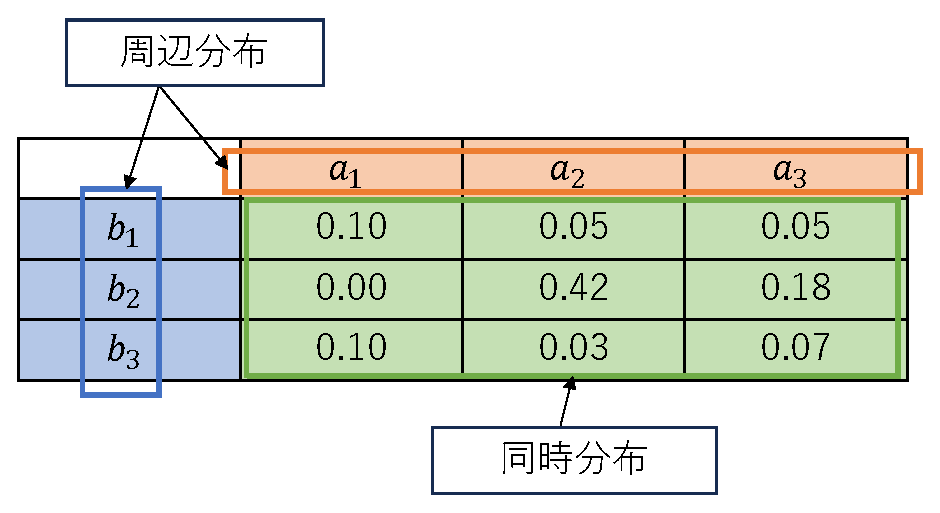
\includegraphics[width=12cm]{figures/fig1.eps} %パスを指定
      \caption{画像タイトル}
      \label{fig:fig_label} %これで引用できる
    \end{figure}

  \subsubsection{表の掲載}
    tableを使います．図と同じようにラベルを参照すれば表\ref{table:table_label}みたいに勝手に番号振ってくれます．
    \begin{table}[h]
      \centering
      \caption{表タイトル}
      \label{table:table_label}
      \begin{tabular}{ccc}
        \hline
          a & b & c\\
          \hline\hline
          1 & 2 & 3\\
        \hline
      \end{tabular}
    \end{table}
  \subsubsection{参考文献の引用}
    このファイルの一番下にthebibliography，その中にbibitemがあり，そこに文献を記載します．例のごとくラベルを参照すれば\cite{cite1}のように勝手に番号振ってくれます．

\newpage % 改ページをするならこれ

\section{セクション2}
  セクションを増やしたりしてゼミ資料を書いてください．

\lhead{参考文献}
\begin{thebibliography}{99}
  \bibitem{cite1}
  参考文献1
  \bibitem{cite2}
  参考文献2
\end{thebibliography}

\end{document}